% KU Leuven latex presentation template
%
% © 2012 Michael Hofmann
%
% This work is licensed under the Creative Commons Attribution 3.0 Unported License.
% To view a copy of this license, visit
% http://creativecommons.org/licenses/by/3.0/ or send a letter to Creative
% Commons, 444 Castro Street, Suite 900, Mountain View, California, 94041, USA.

\documentclass[t,12pt,english
\ifx\beamermode\undefined\else,\beamermode\fi
]{beamer}
%\setbeameroption{show notes}
%\setbeameroption{show only notes}

\usepackage[utf8]{inputenc}
\usepackage[T1]{fontenc}
\usepackage{amsmath}
\usepackage[nohyperlinks]{acronym}
\usepackage{babel,lmodern,graphicx,mathptmx,xspace,wasysym,microtype,booktabs,tabularx,relsize,textcomp,longtable,lipsum,colortbl,eurosym,url,multicol,etoolbox,multimedia,pdfpages,fixltx2e,ifluatex,epstopdf}
\usepackage[olditem,oldenum]{paralist}
\usepackage[babel=true]{csquotes}
\usepackage[thinqspace,amssymb,textstyle]{SIunits}
\usepackage[textsize=tiny]{todonotes}
\usepackage[symbol]{footmisc}
\usepackage[notquote]{hanging}
\usepackage[normalem]{ulem}
%\usepackage{lua-visual-debug}

\pdfstringdefDisableCommands{\renewcommand{\sout}{}}
\graphicspath{{Images/}}
% Fix sort order in case the same file exists with multiple extensions
\DeclareGraphicsExtensions{.pdf,.png,.jpeg,.jpg,.eps}
\frenchspacing

\input{templates/definitions.tex}



%% From pandoc default template
%% End pandoc

\mode<presentation>

%\hypersetup{pdfpagemode=FullScreen}

\definecolor{kuldefault}{HTML}{00407a}
\definecolor{kulbright}{HTML}{52bdec}
\definecolor{kulleft}{HTML}{1d8db0}
\definecolor{kulright}{HTML}{116e8a}

\definecolor{kulyellow}{HTML}{BC8F00}
\definecolor{kulorange}{HTML}{BC6E00}
\definecolor{kulgreen}{HTML}{007F4F}
\definecolor{kulred}{HTML}{FF4422}

\setbeamercolor{structure}{fg=kulbright}
\setbeamercolor{title}{fg=white}
\setbeamercolor{footline}{parent=title}
\setbeamercolor{normal text}{fg=kuldefault}
\setbeamercolor{item}{parent=normal text}
\setbeamercolor{section in toc}{parent=normal text}
\setbeamerfont{title}{size=\Large}
\setbeamerfont{tiny structure}{series=\bfseries}
\setbeamerfont{caption}{}

\setbeamersize{text margin left=0.8cm}
\setbeamersize{text margin right=0.8cm}
\setbeamersize{sidebar width left=0cm}

\setbeamertemplate{navigation symbols}{}
\setbeamertemplate{itemize item}{\footnotesize\raise1pt\hbox{\textbullet}}
\setbeamertemplate{itemize subitem}{--}
\setbeamertemplate{itemize subsubitem}{\tiny\raise1.5pt\hbox{\textbullet}}

\setlength\leftmargini{1em}
\setlength\leftmarginii{1em}
\setlength\leftmarginiii{1em}

\defbeamertemplate{background canvas}{title}
{%
    \pgfdeclarehorizontalshading{bgshading}{8.70cm}{color(0cm)=(kulleft); color(\the\paperwidth)=(kulright)}%
    \vbox to 8.70cm{%
        \pgfuseshading{bgshading}\hspace*{-1.6cm}%
    }%
    \hskip-\paperwidth%
    \hskip1.6cm%
    \vbox to \paperheight{%
        \vskip0.5cm\hskip0.5cm\includegraphics[width=2.83cm]{templates/kuleuven}%
        \vskip0.99cm\hskip0.76cm\includegraphics[width=2.84cm]{templates/key}%
        \vskip-0.57cm\hskip11.61cm\includegraphics[width=0.58cm]{templates/sedes}\hspace*{-1cm}%
        \vfill
    }%
}

\defbeamertemplate{background canvas}{grid}
{%
    \begin{tikzpicture}[remember picture,overlay,every node/.style={anchor=center}]
        \foreach \d in {0,...,20} {
            \draw[gray] (\d,0) -- (\d,-20);
            \draw[gray] (0,-\d) -- (20,-\d);
            \draw[lightgray] (\d+0.5,0) -- (\d+0.5,-20);
            \draw[lightgray] (0,-\d-0.5) -- (20,-\d-0.5);
            \node[anchor=north,red,font=\tiny] at (\d,0) {\d};
            \node[anchor=west,red,font=\tiny] at (0,-\d) {\d};
        }
    \end{tikzpicture}
}

\defbeamertemplate{background canvas}{plain}{}

\defbeamertemplate{footline}{large}
{%
    \pgfdeclarehorizontalshading{bgshading}{0.62cm}{color(0cm)=(kulleft); color(\the\paperwidth)=(kulright)}%
    \vskip.3cm% make room for the logo
    \parbox[t][0.62cm]{\paperwidth}{\pgfuseshading{bgshading}}\par%
    \vskip-0.62cm%
    \begin{beamercolorbox}[ht=0.37cm,dp=0.25cm,center]{page number in head/foot}%
    \insertframenumber%
    \end{beamercolorbox}%
    \vskip-0.92cm%
    \parbox[t][0.92cm]{\paperwidth}{\hskip10.33cm\includegraphics[width=2.10cm]{templates/kuleuven}}\par%
}

\defbeamertemplate{footline}{nopagenumber}
{%
    \pgfdeclarehorizontalshading{bgshading}{0.62cm}{color(0cm)=(kulleft); color(\the\paperwidth)=(kulright)}%
    \vskip.3cm% make room for the logo
    \parbox[t][0.62cm]{\paperwidth}{\pgfuseshading{bgshading}}\par%
    \vskip-0.62cm%
    \begin{beamercolorbox}[ht=0.37cm,dp=0.25cm,center,ignorebg]{page number in head/foot}%
    %
    \end{beamercolorbox}%
    \vskip-0.92cm%
    \parbox[t][0.92cm]{\paperwidth}{\hskip10.33cm\includegraphics[width=2.10cm]{templates/kuleuven}}\par%
}

\defbeamertemplate{footline}{small}
{%
    \vskip.3cm% make room for the logo
    \begin{beamercolorbox}[ht=0.37cm,dp=0.25cm,center,ignorebg]{normal text}%
    \mdseries\insertframenumber%
    \end{beamercolorbox}%
}

\setbeamertemplate{footline}[large]

\setbeamertemplate{frametitle}
{%
    \nointerlineskip%
    \vskip.28cm%
    {\usebeamercolor[fg]{framesubtitle}\usebeamerfont{framesubtitle}\insertsupertitle\strut\par}%
    \vskip-.2cm%
    {\usebeamercolor[fg]{frametitle}\usebeamerfont{frametitle}\insertframetitle\strut\par}%
    \vskip-.3cm%
}

\setbeamertemplate{title page}
{
    \vbox{}%
    \vskip2.8cm%
    \vbox to 6.5cm{%
        \hskip2.8cm%
        \begin{minipage}{7.9cm}
            \begin{beamercolorbox}{title}
                \usebeamerfont{title}%
                \inserttitle\par%
                \ifx\insertsubtitle\undefined%
                \else%
                    \vskip0.25em%
                    {\usebeamerfont{subtitle}\usebeamercolor[fg]{subtitle}\insertsubtitle\par}%
                \fi%
            \end{beamercolorbox}%
            \vskip1em\par
            \begin{beamercolorbox}{author}
                \usebeamerfont{author}\usebeamercolor[fg]{subtitle}%
                \insertauthor
            \end{beamercolorbox}
            \begin{beamercolorbox}{institute}
                \usebeamerfont{institute}\usebeamercolor[fg]{subtitle}%
                \insertinstitute
                \end{beamercolorbox}
            \begin{beamercolorbox}{date}
                \usebeamerfont{date}\usebeamercolor[fg]{subtitle}%
                \insertdate
            \end{beamercolorbox}%
        \end{minipage}%
        \vfill
    }
}

\mode<all>

\newcommand{\inlinesound}[2]{\movie[inlinesound,encoding=Signed,samplingrate=44100]{#1}{#2}}

% disable for now as otherwise all commands that go between frames generated by
% the filter will result in duplicate toc lines
\renewcommand{\addcontentsline}[3]{}

\newcommand{\largefooter}{\setbeamertemplate{footline}[large]}
\newcommand{\emptyfooter}{\setbeamertemplate{footline}[nopagenumber]}
\newcommand{\smallfooter}{\setbeamertemplate{footline}[small]}

\newcommand{\sectiontoc}{\AtBeginSection[]{{
    \nosupertitle
    \emptyfooter
    \begin{frame}[noframenumbering]{Outline}
                \tableofcontents[currentsection]
            \end{frame}
    \largefooter
}}}

\newcommand{\subsectiontoc}{\AtBeginSubsection[]{{
    \nosupertitle
    \emptyfooter
    \begin{frame}[noframenumbering]{Outline}
                \tableofcontents[currentsection,currentsubsection]
           \end{frame}
    \largefooter
}}}

\newcommand{\notoc}{\AtBeginSection[]{}\AtBeginSubsection[]{}}

\newcommand{\nosupertitle}{\renewcommand{\insertsupertitle}{}}
\newcommand{\sectiontitle}{\renewcommand{\insertsupertitle}{\insertsectionhead}}
\newcommand{\subsectiontitle}{\renewcommand{\insertsupertitle}{\insertsectionhead\ifx\insertsubsectionhead\empty\else{} -- \insertsubsectionhead\fi}}

% animations do not work atm as figures are set on independent frames
\newcommand{\slidefig}[2]{\usebackgroundtemplate{\parbox[c][\paperheight][c]{\paperwidth}{\centering\includegraphics#1[height=\paperheight,width=\paperwidth,keepaspectratio]{#2}}}\begin{frame}[plain]\end{frame}\usedefaultcanvas}

\newcommand{\usedefaultcanvas}{\setbeamertemplate{background canvas}[\defaultcanvas]}
\newcommand{\gridcanvas}{\renewcommand{\defaultcanvas}{grid}\usedefaultcanvas}
\newcommand{\plaincanvas}{\renewcommand{\defaultcanvas}{plain}\usedefaultcanvas}

\newcommand{\insertsupertitle}{}






\newcommand{\defaultcanvas}{plain}


% Defining a new coordinate system for the page:
%
% ----------------
% |(0,1)    (1,1)|
% |              |
% |(0,0)    (1,0)|
% ----------------
\makeatletter
\def\parsecomma#1,#2\endparsecomma{\def\page@x{#1}\def\page@y{#2}}
\tikzdeclarecoordinatesystem{page}{
    \parsecomma#1\endparsecomma
    \pgfpointanchor{current page}{north east}
    % Save the upper right corner
    \pgf@xc=\pgf@x%
    \pgf@yc=\pgf@y%
    % save the lower left corner
    \pgfpointanchor{current page}{south west}
    \pgf@xb=\pgf@x%
    \pgf@yb=\pgf@y%
    % Transform to the correct placement
    \pgfmathparse{(\pgf@xc-\pgf@xb)*\page@x+(\pgf@xb)}
    \expandafter\pgf@x\expandafter=\pgfmathresult pt
    \pgfmathparse{(\pgf@yc-\pgf@yb)*\page@y+(\pgf@yb)}
    \expandafter\pgf@y\expandafter=\pgfmathresult pt
}
\makeatother

% Example:
%\begin{tikzpicture}[remember picture,overlay,every node/.style={anchor=center}]
%  \node at (page cs:0.5,0.3) {0.5,0.3};
%  \node at (page cs:0,0) {0,0};
%  \draw(page cs:0,0) -- (page cs:1,1);
%  \draw[thick,red] (page cs:0,0) rectangle (page cs:1,1);
%  \draw[thick,green] (page cs:0.2,0.2) rectangle (page cs:0.8,0.8);
%\end{tikzpicture}

\setcounter{secnumdepth}{0}

\title{Ultra Fast Cardiovascular Imaging}
\subtitle{\tiny Radiation and matter presentation course }
\author{\\ \href{vangjush.komini@uzleuven.be}{\textbf{\textit{Vangjush Komini}}}
}


\institute{{\tiny }\vspace{.10cm} }
\date{\href{www.kul.be}{KU Leuven}\\ \vspace{.10cm}\today}

\begin{document}

\setbeamertemplate{background canvas}[title]

\begin{frame}[plain,noframenumbering]
    \titlepage
\end{frame}

\usedefaultcanvas


\emptyfooter
\begin{frame}[noframenumbering]{Outline}
        \tableofcontents
    \end{frame}
\largefooter

\section{Heart}\label{first-section}



\begin{frame}{Heart}


\begin{figure}[!htb]
\minipage{0.5\textwidth}

\begin{block}{\footnotesize{Facts}}\tiny{}
\begin{enumerate} 
\vspace{0.05cm}
     \item \tiny{\textbf{\textit{Heart diseases the leading death worldwide}}} 
     \item \tiny{\textbf{\textit{No social, economical, demographics associations.}}}
     \item \tiny{\textbf{\textit{5M Americans with heart disease in 2006\cite{3}}}} 
     
\end{enumerate}
\end{block}
     


\begin{block}{\footnotesize{\tiny Early diagnostics the best treatment}}\tiny{}
\begin{enumerate} 
\vspace{0.05cm}
     \item \tiny{\textbf{\textit{Abundant information withing a cardiac cardiac cycle}}} 
     \item \tiny{\textbf{\textit{Heart rate relatively high \textit{\textbf{1.2 beats/s}}}}}\\ 
     \item \tiny{\textbf{\textit{Heart rate variability still a challenge}}}\\ 
   
\end{enumerate}
\end{block}

\endminipage
\minipage{0.5\textwidth}
\centering
\includegraphics[width=.6\textwidth]{1.jpg}\\
\includegraphics[width=.65\textwidth]{2.jpg}\\


\endminipage
\end{figure}

\end{frame}

\begin{frame}{Need for speed}


\begin{figure}[!htb]
\minipage{0.5\textwidth}

\begin{block}{\footnotesize{Decent Ultrasound System}}\tiny{}
\begin{enumerate} 
\vspace{0.05cm}
     \item \tiny{\textbf{\textit{Heart morphology}}}
     \item \tiny{\textbf{\textit{Approximate kinematic}}} 
     \item \tiny{\textbf{\textit{Overall motion estimation}}}
     \color{red} 
     \item \tiny{\textbf{\textit{Time resolution not enough for brief cardiac event}}}
     \item \tiny{\textbf{\textit{Important information can't be be retrieved within a heart beat}}}
     \item \tiny{\textbf{\textit{3D images a must for accurate diagnostic}}}\\
\end{enumerate}
\end{block}
\color{red} 
\tiny{The speed does not meet important functional requirements!}  
\begin{block}{\footnotesize{Research goal}}\tiny{}
\begin{enumerate} 
\vspace{0.05cm}
     \item \tiny{\textbf{\textit{Significant frame rate improvement 30Hz->500 Hz}}}
   
\end{enumerate}
\end{block}

\includegraphics[width=.6\textwidth]{5.jpg}\\
\endminipage
\minipage{0.5\textwidth}
\centering
\includegraphics[width=.6\textwidth]{3.jpg}\\
\includegraphics[width=.6\textwidth]{4.jpg}\\


\endminipage
\end{figure}
\end{frame}

\section{Ultrasound imaging}

\begin{frame}{Benchmark}


\begin{figure}[!htb]
\minipage{0.3\textwidth}

\begin{block}{\footnotesize{Data acquisition}}\tiny{}
\begin{enumerate} 
\vspace{0.05cm}
     \color{red}
     \item \tiny{\textbf{\textit{Pulse-echo measurement}}}
\end{enumerate}
\end{block}

\begin{block}{\footnotesize{Image reconstruction}}\tiny{}
\begin{enumerate} 
\vspace{0.05cm}
     \item \tiny{\textbf{\textit{RF filtering}}}
     \item \tiny{\textbf{\textit{Envelope detection}}}
     \item \tiny{\textbf{\textit{Attenuation correction}}}
     \item \tiny{\textbf{\textit{Log compression}}}
     \item \tiny{\textbf{\textit{Scan conversion}}}
\end{enumerate}
\end{block}

\endminipage
\minipage{0.7\textwidth}
\centering

\includegraphics[width=.51\textwidth]{18.jpg}

\endminipage
\end{figure}

\end{frame}



\begin{frame}{Ultrasound path}

\begin{figure}[!htb]
\minipage{0.5\textwidth}
\includegraphics[width=.7\textwidth]{19.jpg}\\
\includegraphics[width=.7\textwidth]{22.jpg}\\
\tiny Axial resolution:$\Delta x=\frac{c}{2\Delta B_{Pulse}}$\\
\tiny Lateral resolution:$\Delta z=\frac{\lambda_{c}D)_{f}}{a^{tx}+a^{rx}}$
\endminipage
\minipage{0.55\textwidth}
\centering

\includegraphics[width=.7\textwidth]{20.jpg}\\
\includegraphics[width=.4\textwidth]{24.jpg}\\
\includegraphics[width=.4\textwidth]{25.jpg}\\

\endminipage
\end{figure}

\end{frame}



\begin{frame}{Benchmark}


\begin{figure}[!htb]
\minipage{0.3\textwidth}

\begin{block}{\footnotesize{Data acquisition}}\tiny{}
\begin{enumerate} 
\vspace{0.05cm}
    
     \item \tiny{\textbf{\textit{Pulse-echo measurement}}}
\end{enumerate}
\end{block}

\begin{block}{\footnotesize{Image reconstruction}}\tiny{}
\begin{enumerate} 
\vspace{0.05cm}
     \color{red}
     \item \tiny{\textbf{\textit{RF filtering}}}
     \item \tiny{\textbf{\textit{Envelope detection}}}
     \item \tiny{\textbf{\textit{Attenuation correction}}}
     \item \tiny{\textbf{\textit{Log compression}}}
     \item \tiny{\textbf{\textit{Scan conversion}}}
\end{enumerate}
\end{block}
\endminipage
\minipage{0.7\textwidth}
\centering
\includegraphics[width=.31\textwidth]{27.jpg}\\
\includegraphics[width=.31\textwidth]{6-1.jpg}\\
\includegraphics[width=.31\textwidth]{7.jpg}\\

\endminipage


\end{figure}

\end{frame}

\begin{frame}{Benchmark}


\begin{figure}[!htb]
\minipage{0.3\textwidth}

\begin{block}{\footnotesize{Data acquisition}}\tiny{}
\begin{enumerate} 
\vspace{0.05cm}
    
     \item \tiny{\textbf{\textit{Pulse-echo measurement}}}
\end{enumerate}
\end{block}

\begin{block}{\footnotesize{Image reconstruction}}\tiny{}
\begin{enumerate} 
\vspace{0.05cm}
     \color{red}
     \item \tiny{\textbf{\textit{RF filtering}}}
     \item \tiny{\textbf{\textit{Envelope detection}}}
     \item \tiny{\textbf{\textit{Attenuation correction}}}
     \item \tiny{\textbf{\textit{Log compression}}}
     \item \tiny{\textbf{\textit{Scan conversion}}}
\end{enumerate}
\end{block}
\endminipage
\minipage{0.7\textwidth}
\centering
\includegraphics[width=.31\textwidth]{8.jpg}\\
\includegraphics[width=.31\textwidth]{6.jpg}\\
\includegraphics[width=.31\textwidth]{28.jpg}\\

\endminipage


\end{figure}

\end{frame}


\begin{frame}{Speeding up acquisition}



\begin{figure}[!htb]
\minipage{0.5\textwidth}

\begin{equation}
\tiny FrameRate=\frac{1}{Nr_{tx}\Delta ToF}
\end{equation}
\begin{block}{\footnotesize{Time of flight~}}\tiny{}
\begin{enumerate} 
\vspace{0.05cm}
     \item \tiny{\textbf{\textit{Speed of sound in tissue \tiny{$1540 m/s$}}}}
     \item \tiny{\textbf{\textit{Propagation distance depth \tiny{$30 cm$}}}}
     \item \tiny{\textbf{\textit{Duration for a single line \tiny{$200 \mu s$}}}}
\end{enumerate}
\end{block}

\begin{block}{\footnotesize{Number of beams transmitted}}\tiny{}
\begin{enumerate} 
\vspace{0.05cm}
     \item \tiny{\textbf{\textit{Minimum number of beams for a sector image is $200$}}}
     \item \tiny{\textbf{\textit{Frame rate achieved $25 F/s$.}}}
\end{enumerate}
\end{block}

\endminipage
\minipage{0.7\textwidth}
\centering
\includegraphics[width=.5\textwidth]{11.jpg}\\

\endminipage

\begin{itemize}
\color{red}
\item \small ToF and the sound velocity restricted by the matter and the depth.
\item \small Number of transmit event needs to be reduced for high frame rate. 
\end{itemize}

\end{figure}

\end{frame}



\section{How to go fast.}


\begin{frame}{Lowering transmit events}

\begin{itemize}
\color{red}
\item \tiny{Reduction of line density is not a solution because it reduces the image quality.}  
\end{itemize}



\begin{block}{\footnotesize{Possible candidates}}\tiny{}
\begin{enumerate} 
\vspace{0.05cm}
     \item \tiny{\textbf{\textit{Retrospective Gating}}}
     \item \tiny{\textbf{\textit{Multi-Line-Acquisition}}}
     \item \tiny{\textbf{\textit{Multi-Line-Transmission}}}
\end{enumerate}
\end{block}


\end{frame}

\begin{frame}{Retrospective Gating}


\begin{figure}[!htb]
\minipage{0.5\textwidth}
\begin{block}{\footnotesize{}}\tiny{}
\begin{enumerate} 
\vspace{0.05cm}

     \item \tiny{\textbf{\textit{Region of interest is divided into small sectors}}}
     \item \tiny{\textbf{\textit{Each sectors is scanned at high rate}}}
     \item \tiny{\textbf{\textit{The sector images are then combined at the end}}}

\end{enumerate}
\end{block}

\begin{block}{\footnotesize{\tiny Preserve \textit{image quality} and FoV\cite{3}}}\tiny{}
\begin{enumerate} 
\vspace{0.05cm}
\color{red}
     \item \tiny{\textbf{\textit{Inaccuracy due to HRV}}}
     \item \tiny{\textbf{\textit{Breathing also affect the heart positioning}}}
     \item \tiny{\textbf{\textit{Gating via ECG}}}
     \item \tiny{\textbf{\textit{Not possible withing a single beat}}}

\end{enumerate}
\end{block}

\endminipage
\minipage{0.5\textwidth}
\centering
\includegraphics[width=1.2\textwidth]{13.jpg}
\endminipage
\end{figure}


\end{frame}


\begin{frame}{MLA }


\begin{figure}[!htb]
\minipage{0.5\textwidth}


\begin{block}{\footnotesize{\tiny Reduced aperture\cite{4}}}\tiny{}
\begin{equation}
N_{mla}=\frac{p^{tx}}{p^{txrx}}(1+\frac{a^{rx}}{a^{tx}})
\end{equation}
\begin{enumerate} 
\vspace{0.05cm}

     \item \tiny{\textbf{\textit{Parallel receive beamforming from RoI}}}
     \item \tiny{\textbf{\textit{X-fold the acquisition time}}}
     \item \tiny{\textbf{\textit{Broadening the transmit field via smaller aperture}}}
     \color{red}
     \item \tiny{\textbf{\textit{Less energy transmitted, particularly into larger depth, decayed SNR}}}
     \item \tiny{\textbf{\textit{Broadening the beam outcomes a smaller lateral and spatial resolution}}}
     \item \tiny{\textbf{\textit{Stationary stripes along the direction of ultrasound beam at the end}}}
     
\end{enumerate}
\end{block}
\includegraphics[width=.5\textwidth]{14.jpg}\\
\endminipage
\minipage{0.5\textwidth}
\centering
\includegraphics[width=.4\textwidth]{div.jpg}\\
\includegraphics[width=.4\textwidth]{open.jpg}\\
\includegraphics[width=.5\textwidth]{MLAresults2.jpg}\\
\caption{\tiny Field-II simulation}
\endminipage
\end{figure}


\end{frame}


\begin{frame}{MLA  }


\begin{figure}[!htb]
\minipage{0.5\textwidth}


\begin{block}{\footnotesize{\tiny Plane wave or diverging wave \cite{1}}}\tiny{}
\begin{enumerate} 
\vspace{0.05cm}

     \item \tiny{\textbf{\textit{It uses the full aperture}}}
     \item \tiny{\textbf{\textit{Higher number of parallel receive beams}}}
     \item \tiny{\textbf{\textit{Good energy penetration}}}
     \item \tiny{\textbf{\textit{4-MLA is a recommended threshold}}}
     \color{red}
     \item \tiny{\textbf{\textit{Spatial resolution is decreased significantly from the broader beam}}}
     \item \tiny{\textbf{\textit{Diverging waves perform even poorer than plane waves}}}
     
\end{enumerate}
\end{block}
\endminipage
\minipage{0.4\textwidth}
\centering
\includegraphics[width=.7\textwidth]{platewave.jpg}\\
\includegraphics[width=.7\textwidth]{MLAresults1.jpg}\\
\endminipage
\end{figure}


\end{frame}

\begin{frame}{MLA }


\begin{figure}[!htb]
\minipage{0.5\textwidth}


\begin{block}{\footnotesize{\tiny Spatial compounding \cite{5}}}\tiny{}
\begin{enumerate} 
\vspace{0.05cm}

     \item \tiny{\textbf{\textit{RoI imaged from two beams}}}
     \item \tiny{\textbf{\textit{The overlap is averaged}}}
     \item \tiny{\textbf{\textit{Significant improvement of image quality }}}
     \color{red}
     \item \tiny{\textbf{\textit{Requires higher number of beams}}}
     \item \tiny{\textbf{\textit{Could induce motion artifacts}}}
     \item \tiny{\textbf{\textit{Via diverging waves the gain frame rate could be increased}}}
     \item \tiny{\textbf{\textit{Harmonic imaging almost impossible due to low pressure reaching the region. Fading of higher harmonics}}}
     
\end{enumerate}
\end{block}
\endminipage
\minipage{0.4\textwidth}
\centering
\includegraphics[width=1\textwidth]{Compounding.jpg}\\
\includegraphics[width=.5\textwidth]{Compounding1.jpg}\\
\endminipage
\end{figure}


\end{frame}



\begin{frame}{MLT}


\begin{figure}[!htb]
\minipage{0.5\textwidth}


\begin{block}{\footnotesize{\tiny A step further \cite{6}}}\tiny{}
\begin{enumerate} 
\vspace{0.05cm}
     \item \tiny{\textbf{\textit{Much higher temporal resolution}}}
     \item \tiny{\textbf{\textit{Broadening the beam, not a must}}}
     \item \tiny{\textbf{\textit{Combined with MLA could potentially increase the gain frame rate}}}
     \item \tiny{\textbf{\textit{Harmonic imaging is feasible}}}
\color{red}
     \item \tiny{\textbf{\textit{Little attention due to cross talking}}}
      \item \tiny{\textbf{\textit{Apodization, orthogonality could tackle cross-talking}}}
      \item \tiny{\textbf{\textit{Depends significantly on the system configuration}}}
\end{enumerate}
\end{block}
\endminipage
\minipage{0.5\textwidth}
\centering
\includegraphics[width=.5\textwidth]{17.jpg}\\
\includegraphics[width=.5\textwidth]{12.jpg}\\
\endminipage
\end{figure}


\end{frame}


\begin{frame}{MLT}

Single line pressure field
\tiny{$$p({\mathop{r}\limits^{\rightharpoonup}},t)=\rho_{0}{\partial v(t) \over \partial t}\ast\sum_{i=1}^{N}w_{i}^{{\rm xmt}}h_{i}({\mathop{r}\limits^{\rightharpoonup}},t+\Delta t_{i}^{{\rm xmt}}).\eqno{\hbox{(2)}}$$}
\small Received echo signal base
\tiny{$$\eqalignno{E(t)=& {q\rho_{0}a \over 2}{\partial \over \partial t}\left[{p({\mathop{r}\limits^{\rightharpoonup}},t) \over \rho_{0}^{C}}\right]\ast\sum_{j=1}^{N}w_{j}^{{\rm rcv}}(t)\cdot h_{j}({\mathop{r}\limits^{\rightharpoonup}},t+\Delta t_{j}^{{\rm r}\alpha}(t))\cr=$$

\tiny{$$& {qa\rho_{0} \over 2c}{\partial^{2}v(t) \over \partial t^{2}}\ast\left[\sum_{i=1}^{N}w_{i}^{{\rm xmt}}h_{i}({\mathop{r}\limits^{\rightharpoonup}},t+\Delta t_{i}^{{\rm xmt}})\right] \cr & \ast \left[\sum_{j=1}^{N} w_{j}^{{\rm rev}}(t)\cdot h_{j}({\mathop{r}\limits^{\rightharpoonup}},t+\Delta t_{j}^{{\rm rcv}}(t))\right], & \hbox{(3)}}$$}}

\end{frame}


\begin{frame}{MLT}

\begin{figure}[!htb]
\minipage{0.5\textwidth}
\begin{block}{\footnotesize{\tiny }}\tiny{}
\begin{enumerate} 
\vspace{0.05cm}

     \item \tiny{\textbf{\textit{Aperture is divided into several apertures}}}
     \item \tiny{\textbf{\textit{One of the sub aperture generating one of the beams}}}
     \item \tiny{\textbf{\textit{Suporimposing multimple delay map yield MLT}}}
\color{green}
     \item \tiny{\textbf{\textit{On transmit aperture appropriate apodization could be used to generate more than one beam at single pulse}}}\\
\includegraphics[width=.7\textwidth]{MLT.jpg}\\
\end{enumerate}
\end{block}
\endminipage
\minipage{0.5\textwidth}
\centering
\includegraphics[width=1\textwidth]{MLT_beamforming1.jpg}\\
\includegraphics[width=1\textwidth]{MLTpressure.jpg}\\
\caption{ \tiny{Pressure profile \cite{6}}}
\endminipage
\end{figure}

\end{frame}




\begin{frame}{MLT}

\small Single line pressure field

\tiny{$$\eqalignno{p_{2{\rm mlt}}({\mathop{r}\limits^{\rightharpoonup}}, t) = & \rho_{0}{\partial v(t) \over \partial t}\ast\sum_{i=1}^{N}[w_{i}^{1,{\rm xmt}}h_{i}({\mathop{r}\limits^{\rightharpoonup}}, t+\Delta t_{i}^{1,{\rm xmt}})\cr & +w_{i}^{2,{\rm xmt}}h_{i}({\mathop{r}\limits^{\rightharpoonup}},t+\Delta t_{i}^{2,{\rm xmt}})],& \hbox{(4)}}$$}

\small Received echo signal base


\tiny{$$\eqalignno{E_{2{\rm mlt}}(t)= & {q\rho_{0}a \over 2}{\partial \over \partial t}\cr & \times\left[{p_{2{\rm mlt}}(\hat{r},t) \over \rho_{0}{c}} \ast\sum_{j=1}^{N}w_{j}^{1,{\rm rcv}}(t)\cdot h_{j}({\mathop{r}\limits^{\rightharpoonup}},t+\Delta t_{j}^{1,{\rm rcv}}(t))\right]\cr$$}
\tiny{$$= & {qa\rho_{0} \over 2c}{\partial^{2}v(t) \over \partial t^{2}}\ast\left[\sum_{i=1}^{N} w_{i}^{1,{\rm xmt}}h_{i}({\mathop{r}\limits^{\rightharpoonup}},t+\Delta t_{i}^{1,{\rm xmt}})\right]\cr & \ast\left[\sum_{j=1}^{N}w_{j}^{1,{\rm rcv}}(t)\cdot h_{j}({\mathop{r}\limits^{\rightharpoonup}}, t+\Delta t_{j}^{1,{\rm rcv}}(t))\right]\cr &$$}
\tiny{$$ +{qa\rho_{0} \over 2c}{\partial^{2}v(t) \over \partial t^{2}}\ast\left[\sum_{i=1}^{N}w_{i}^{2,{\rm xmt}}h_{i}({\mathop{r}\limits^{\rightharpoonup}}t+\Delta t_{i}^{2,{\rm xmt}})\right]\cr & \ast\left[\sum_{j=1}^{N}w_{j}^{1,{\rm rcv}}(t)\cdot h_{j}({\mathop{r}\limits^{\rightharpoonup}},t+\Delta t_{j}^{1,{\rm rcv}}(t))\right].& \hbox{(5)}}$$}
\small First term is the echo from the  equivalent SLT whereas the second term is the cross-talk component

\end{frame}






\begin{frame}{MLT}

\begin{figure}[!htb]
\minipage{0.5\textwidth}
\begin{block}{\footnotesize{\tiny }}\tiny{}
\begin{enumerate} 
\vspace{0.05cm}

     \item \tiny{\textbf{\textit{Very good candidate for ultra-fast imaging}}}
     \item \tiny{\textbf{\textit{Competitive image quality with SLT at certain set up}}}
     \item \tiny{\textbf{\textit{Transducer configuration, MLT opening angle, apodization scheme are the main key drivers}}}
     \item \tiny{\textbf{\textit{Extrapolating into 3 imaging is currently ongoing work}}}

\end{enumerate}
\end{block}
\endminipage
\minipage{0.5\textwidth}
\centering
\includegraphics[width=1\textwidth]{MLAresults3.jpg}\\
\includegraphics[width=1\textwidth]{PSF.jpg}\\
\endminipage
\end{figure}

\end{frame}

\begin{frame}{MLT extrapolated into 3D}


\begin{figure}[!htb]
\minipage{0.5\textwidth}
\includegraphics[width=.3\textwidth]{29.jpg}\\
\includegraphics[width=.5\textwidth]{26.jpg}\\
\tiny Aim:\color{red}16MLT*\color{green}4MLA=\color{blue}64 Frame rage gain\\


\endminipage
\minipage{0.5\textwidth}
\centering
\includegraphics[width=1\textwidth]{23.jpg}\\
\endminipage
\end{figure}

\small Experimental validation needed\cite{7}!

\end{frame}


\section{Conclusion}
\begin{frame}{Conclusion}
\begin{itemize}
\item Spatial and temporal resolution in intrinsic relation.
\item Yet there is a plenty of room for improvement! 
\end{itemize}
\end{frame}



\emptyfooter
\begin{frame}{ }
\centering \textbf{\Large \textit{Thank you for your attention!}}
\begin{figure}[!htb]
\includegraphics[width=.3\textwidth]{QA.jpg}
\end{figure}
\largefooter
\end{frame}













\begin{frame}[allowframebreaks]
        \frametitle{References}
        \nocite{*}
        \bibliography{references}
        \bibliographystyle{plain}
\end{frame}

\end{document}